\documentclass[10pt]{article}
\usepackage[utf8]{inputenc}
\usepackage[T1]{fontenc}
\usepackage{graphicx}
\usepackage[export]{adjustbox}
\graphicspath{ {./images/} }
\usepackage{amsmath}
\usepackage{amsfonts}
\usepackage{amssymb}
\usepackage[version=4]{mhchem}
\usepackage{stmaryrd}
\usepackage{hyperref}
\hypersetup{colorlinks=true, linkcolor=blue, filecolor=magenta, urlcolor=cyan,}
\urlstyle{same}

\title{PeopleNet: A Vision for a Decentralized Digital Society }

\author{The PeopleNet Team}
\date{}


\begin{document}
\maketitle
August 10, 2024

\section*{1 Introduction}
In the digital age, blockchain technology has emerged as a beacon of hope, promising a future of decentralization, security, and transparency. However, the dream of a truly decentralized society, especially in regions like India, remains distant. Enter PeopleNet, a project aimed at bridging this gap and bringing blockchain to the masses.

\subsection*{1.1 Vision}
PeopleNet envisions a world where blockchain is accessible to everyone. The primary vision is the mass adoption of blockchain in India. By targeting India, with its diverse and vast population, PeopleNet aims to serve as a truly altruistic network for the greater good.

\subsection*{1.2 Mission}
The mission of PeopleNet is to create a digital society where individuals have full control over their data and financial transactions. In this society, democratic principles flourish in an autonomous, decentralized environment. The goal is to empower individuals, giving them the tools and platform to interact, transact, and govern without intermediaries.

\subsection*{1.3 Goals and Milestones}
PeopleNet sets forth a significant milestone:

\begin{itemize}
  \item A Digital Democracy: A society where every individual can participate in decision-making processes, voice their opinions, and truly make a difference.
\end{itemize}

However, its adoption has been slow, especially in developing countries like India. High entry barriers, lack of awareness, and technical complexities have kept it out of reach for the average individual. PeopleNet aims to change this narrative by simplifying blockchain technology and making it accessible to everyone.

The project recognizes the challenges of the current digital landscape, such as data privacy concerns, centralized control, and lack of transparency. By leveraging blockchain technology, PeopleNet seeks to address these issues, offering a platform that is secure, transparent, and user-friendly.

Furthermore, the project understands the importance of community involvement. By incentivizing good actors and penalizing bad ones, PeopleNet ensures a fair and just platform. The project also encourages boundary-less interactions, allowing users to connect, collaborate, and transact seamlessly.

In conclusion, PeopleNet is not just a blockchain project; it's a movement. A movement to democratize technology, empower individuals, and create a truly decentralized digital society.

\section*{2 Problem Statement}
The digital age, while bringing about unprecedented advancements and conveniences, has also ushered in a slew of challenges. Centralization, data monopolies, and a lack of genuine user control over personal data have become the norm rather than the exception. These issues are particularly pronounced in developing nations like India, where the digital divide is still a pressing concern.

\subsection*{2.1 Inaccessibility of Resources}
For the common man in India, the digital world often remains an elusive realm. While urban centers see\\
rapid digitization, vast swathes of the rural landscape remain untouched by the digital revolution. This digital divide means that a significant portion of the population is denied access to the myriad opportunities that the online world offers.

\subsection*{2.2 Capitalism and Global Market Landscape}
The global market landscape is predominantly capitalistic. While capitalism has its merits, it often leads to wealth accumulation in the hands of a few. This economic disparity is starkly evident in the digital realm, where tech giants hold disproportionate power and influence, often at the expense of the average user.

\subsection*{2.3 Inequality and the Need for Facilitation}
The current digital ecosystem is rife with inequality. Whether it's in terms of access to resources, knowledge, or opportunities, the scales are often tipped in favor of a select few. There's a pressing need for a facilitator, a platform that levels the playing field, ensuring that everyone, irrespective of their socio-economic background, has an equal shot at leveraging the digital revolution.

\subsection*{2.4 The Absence of a Truly Altruistic Network}
Most digital platforms operate with profit as the primary motive. While there's nothing inherently wrong with seeking profit, it often comes at the cost of user interests. The digital realm is in dire need of a truly altruistic network, one that places user interests at the forefront, operating not for profit but for the greater good.

In essence, the challenges are manifold. From bridging the digital divide to ensuring a more equitable distribution of digital resources, the need for a transformative solution has never been more urgent.\\
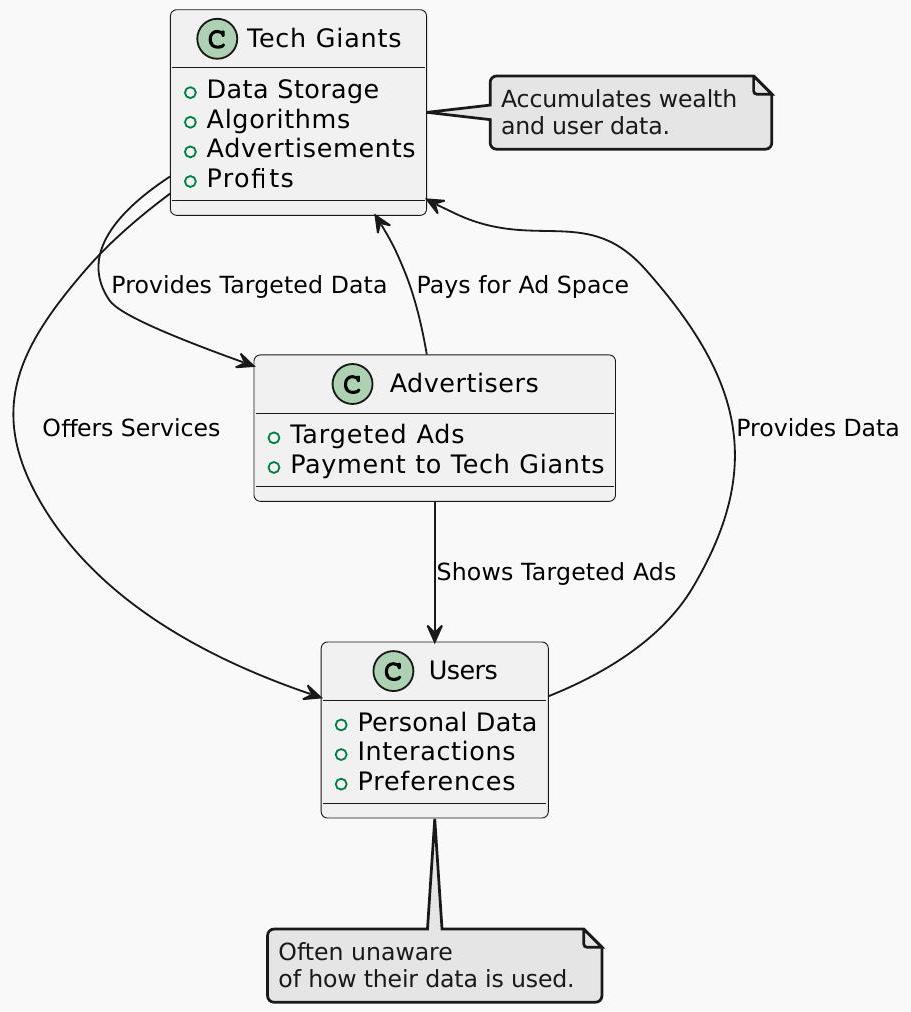
\includegraphics[max width=\textwidth, center]{2025_03_06_545dea0014012947d15fg-02}

Figure 1: Flow of data and profits in the current digital ecosystem.

\section*{3 Current Ethereum Ecosystem}
Ethereum, since its inception, has been a trailblazer in the blockchain world, introducing the concept of smart contracts and decentralized applications (DApps) 11]. However, as the platform grew in popularity, it began facing challenges that are inherent to its design and architecture.

\subsection*{3.1 Scalability}
One of the most pressing issues facing Ethereum today is scalability [9]. As more and more transactions are processed on the network, the time taken to validate and add these transactions to the blockchain increases. This results in a bottleneck, slowing down the entire system and leading to increased transaction fees.

\subsection*{3.2 Gas Fees}
Gas fees on Ethereum have become a significant concern, especially during network congestion [1]. These fees are required to process and validate transactions\\
on the Ethereum network. However, during times of high demand, these fees can skyrocket, making it prohibitively expensive for regular users to make transactions or interact with DApps.

\subsection*{3.3 Decentralization vs. Scalability}
The blockchain trilemma posits that it's challenging to achieve scalability, security, and decentralization all at once [8]. Ethereum, in its quest to maintain decentralization and security, has often faced scalability issues. Solutions like Ethereum 2.0 and layer 2 scaling are in the works to address this, but the trilemma remains a fundamental challenge.

\subsection*{3.4 Transition to Proof-of-Stake}
Ethereum's transition from a Proof-of-Work (PoW) to a Proof-of-Stake (PoS) consensus mechanism is a monumental shift [6]. While PoS promises energy efficiency and scalability, the transition is complex and poses risks, especially concerning network security and validator centralization.

In summary, while Ethereum has paved the way for decentralized applications and smart contracts, it faces challenges that need addressing for it to remain the leading platform for decentralized innovations.

\section*{4 Proposed Solution}
The challenges posed by the current Ethereum ecosystem, especially concerning scalability, gas fees, and decentralization, necessitate an innovative solution. PeopleNet proposes a hybrid model, combining the strengths of zkRollups and Polygon's architecture, to address these challenges.

\section*{4.1 zkRollups}
zkRollups is a layer 2 scaling solution that bundles multiple transfers into a single transaction, reducing the strain on the Ethereum network 13. The primary advantage of zkRollups is its ability to maintain security by inheriting the underlying layer's security guarantees.

The main idea behind zkRollups is the use of zeroknowledge proofs. A zero-knowledge proof allows one party to prove to another party that a statement\\
is true without revealing any information about the statement itself.\\
zkSNARK: $\forall x, y,(P(x)=y) \Longleftrightarrow \exists w, Q(x, w)=y$\\
Where: - $P$ is the program. - $x$ is the public input. - $y$ is the public output. - $w$ is the private witness (or proof).

\subsection*{4.2 Polygon's Architecture}
Polygon's architecture, particularly its emphasis on child chains and the root chain, offers a scalable framework that can handle a vast number of transactions efficiently [16]. The child chains operate independently but are secured by the root chain, ensuring the system's overall security.\\
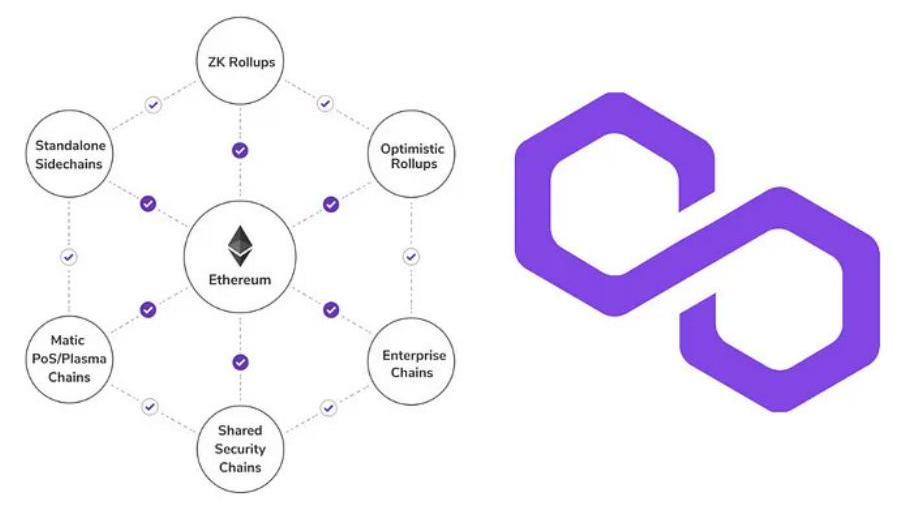
\includegraphics[max width=\textwidth, center]{2025_03_06_545dea0014012947d15fg-03}

Figure 2: Polygon's Root and Child Chain Architecture.

\subsection*{4.3 Hybrid Model: zkRollups + Polygon}
By integrating zkRollups into Polygon's architecture, PeopleNet can achieve high scalability while ensuring security and decentralization. The zkRollups will handle transaction bundling, while Polygon's architecture will manage the hierarchical structure of chains.

This hybrid model will allow for:

\begin{itemize}
  \item Efficient transaction processing.
  \item Reduced gas fees.
  \item Enhanced security through combined strengths.
\end{itemize}

\subsection*{4.4 Incentivizing Good Actors}
One of the unique features of the proposed solution is its mechanism to reward good actors and penalize malicious ones. By integrating a reputation system, users can earn points for positive contributions and lose points for malicious activities.


\begin{equation*}
R_{\text {new }}=R_{\text {old }}+\Delta R \tag{2}
\end{equation*}


Where: - $R_{\text {new }}$ is the new reputation. - $R_{\text {old }}$ is the old reputation. - $\Delta R$ is the change in reputation based on user actions.\\
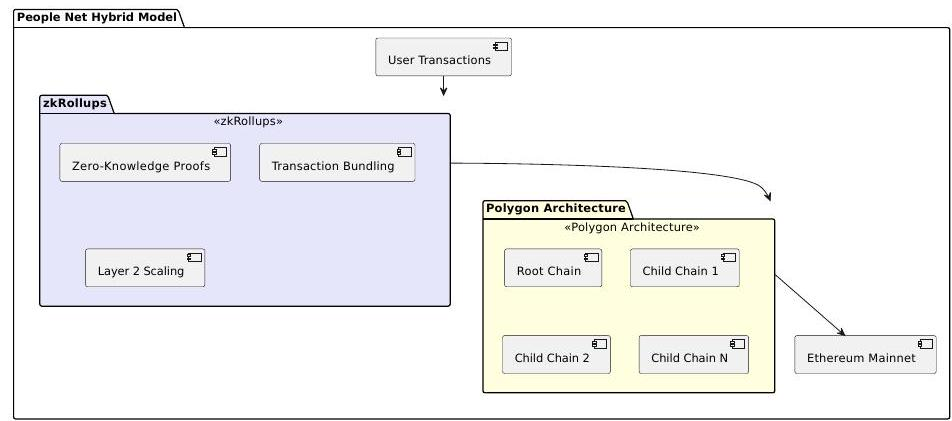
\includegraphics[max width=\textwidth, center]{2025_03_06_545dea0014012947d15fg-04}

Figure 3: PeopleNet's hybrid and Child Chain Architecture.

In conclusion, the proposed hybrid model offers a robust solution to the challenges of the current Ethereum ecosystem. By leveraging the strengths of both zkRollups and Polygon, PeopleNet aims to provide a scalable, secure, and decentralized platform for the masses.

\section*{5 Architecture}
The architecture of PeopleNet is a novel blend, drawing from the strengths of both Polygon's multi-chain framework and zkSync's zkRollups. This section delves deeper into the structure and interactions of the proposed contracts, offering a comprehensive view of the system's design.

\subsection*{5.1 Contract Overview}
The architecture is divided into three primary components:

\begin{itemize}
  \item Polygon: Provides the foundational layer, with contracts like RootChain, ChildChain, and various managers and predicates.
  \item zkSync: Offers scalability through zkRollups, with contracts handling bridging, batched transaction proofs, and validators.
  \item Proposed Architecture: The unique addition to the hybrid model, introducing Macro and Micro chain management, along with AAO factories and managers.
\end{itemize}

\subsection*{5.2 Interactions and Data Flow}
\subsection*{5.2.1 Polygon}
Polygon's RootChain contract serves as the primary entry and exit point for assets. It interacts with the DepositManager for deposits and the WithdrawManager for withdrawals. The respective managers then communicate with predicates to handle specific token types, like ERC20 and ERC721.

\subsection*{5.2.2 zkSync}
zkSync's primary bridge contracts, L1ERC20Bridge and L1WethBridge, interact with the DiamondProxy contract to handle asset bridging. The DiamondProxy, in turn, sends batched transaction proofs to the Plonk4Verifier and manages validator staking through the ValidatorTimelock.

\subsection*{5.2.3 Proposed Architecture}
The MacroChainManager contract serves as the primary management point for the macro chains. It can request the creation of micro-chains through the MicroChainFactory and manage them via the MicroChainManager. Similarly, the MacroAAOFactory and Manager handle the creation and management of macro AAOs, while their micro counterparts handle the micro AAOs.

\subsection*{5.3 Unique Features of the Proposed Architecture}
The proposed architecture introduces a chain-ofchains concept, where each AAO operates as its chain. This hierarchical structure allows for efficient management, scalability, and flexibility. The Macro and Micro managers and factories ensure that AAOs can be created, managed, and operated seamlessly, offering a dynamic environment for various decentralized applications and platforms.\\
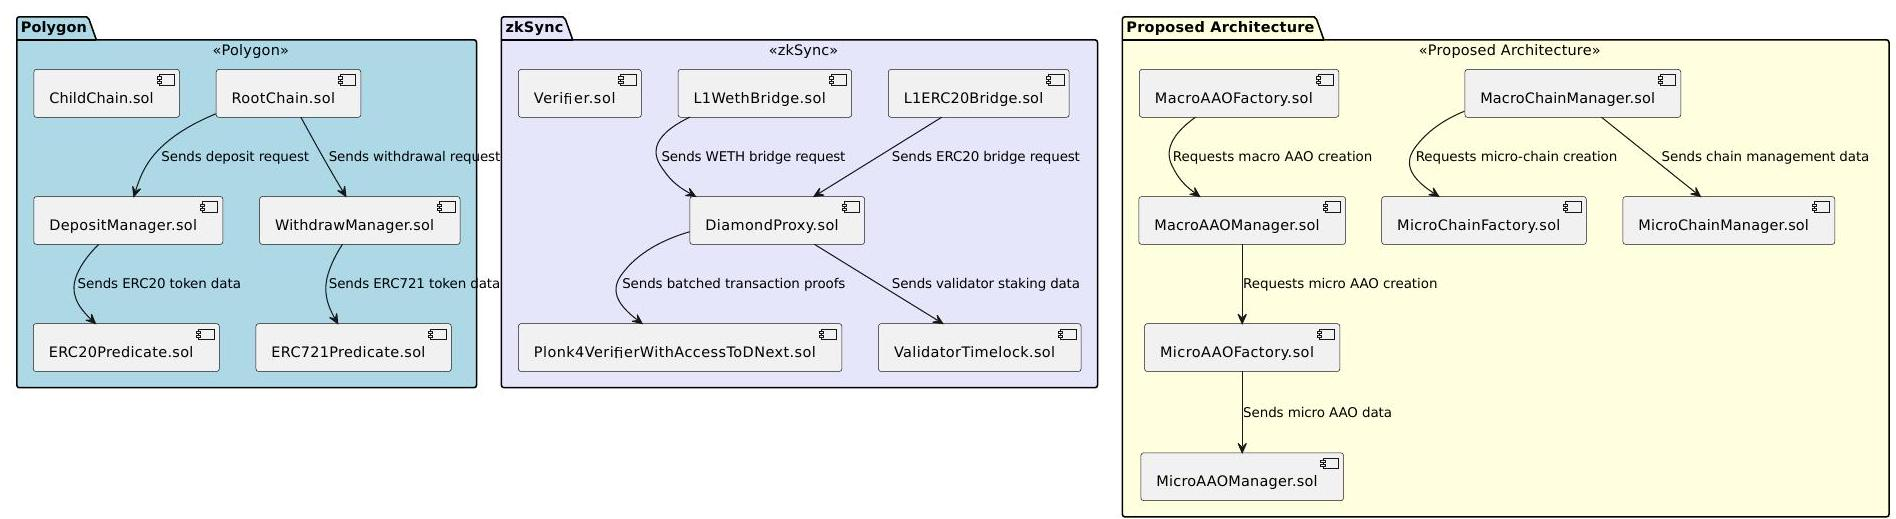
\includegraphics[max width=\textwidth, center]{2025_03_06_545dea0014012947d15fg-05(1)}

Figure 4: Interactions and Data Flow in PeopleNet's Architecture.

In conclusion, the architecture of PeopleNet is a testament to the power of combining established technologies to create a robust, scalable, and secure system, with the flexibility to cater to a wide range of applications.

\section*{6 AAO: Acentric Autonomous Organizations}
Acentric Autonomous Organizations (AAOs) form the backbone of the PeopleNet ecosystem, serving as multipurpose vehicles for online systems. These decentralized entities empower individuals and groups to create, manage, and operate their digital platforms with autonomy, transparency, and security.\\
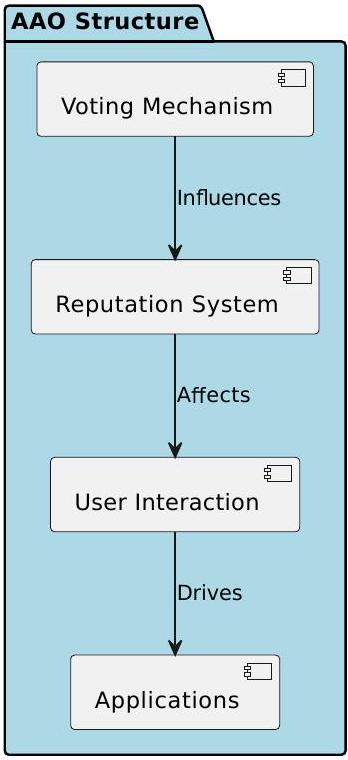
\includegraphics[max width=\textwidth, center]{2025_03_06_545dea0014012947d15fg-05}

Figure 5: Structure and interactions within an AAO.

\subsection*{6.1 Foundational Principles}
AAOs are built upon three foundational principles:

\begin{enumerate}
  \item Autonomy: AAOs operate independently, free from centralized control. Decisions are made collectively by the members, ensuring that the organization's direction aligns with the collective will.
  \item Decentralization: Unlike traditional organizations, AAOs are not bound by hierarchical structures. Power and decision-making are distributed among members, fostering a democratic environment.
  \item Transparency: All operations, transactions, and decisions within an AAO are recorded on the blockchain, ensuring complete transparency and accountability.
\end{enumerate}

\subsection*{6.2 Functionalities and Features}
\subsection*{6.2.1 Voting Mechanisms}
AAOs incorporate decentralized voting mechanisms, allowing members to propose, discuss, and vote on various matters. This ensures that every member has a voice and that decisions reflect the collective consensus.

\subsection*{6.2.2 Reputation Points}
To incentivize positive contributions and deter malicious activities, AAOs employ a reputation system. Members earn or lose reputation points based on their actions, ensuring a meritocratic environment.

\subsection*{6.2.3 User Interaction}
AAOs are not just transactional entities; they are vibrant communities. Members can interact, collaborate, share knowledge, and build relationships, fostering a sense of belonging and community.

\subsection*{6.3 Applications of AAOs}
The versatility of AAOs means they can serve various purposes:

\begin{itemize}
  \item Governance: AAOs can act as decentralized governing bodies, making decisions on community projects, resource allocation, and more.
  \item Entertainment: Artists and creators can form AAOs to produce and distribute content, ensuring fair compensation and creative freedom.
  \item Communication: AAOs can serve as platforms for open discussions, debates, and knowledge sharing, free from censorship and external control.
  \item Funding: Startups and projects can seek funding through AAOs, connecting directly with supporters and bypassing traditional financial intermediaries.
\end{itemize}

In conclusion, AAOs represent a paradigm shift in how we conceive organizations. By prioritizing autonomy, decentralization, and transparency, they offer a blueprint for the future of online communities and platforms.

\section*{7 Tokenomics}
The PeopleNet ecosystem introduces a unique token system designed to facilitate transactions, incentivize positive behavior, and ensure the smooth operation of the platform. The tokenomics revolves around three primary tokens: KAS, REP, and PNT (12].

\subsection*{7.1 KAS: The Primary Currency}
KAS serves as the main currency within the PeopleNet ecosystem. Pegged to the Indian Rupee, it ensures stability and familiarity for the Indian user base. The token is used for financial transactions\\
within the network and is bridged with its Ethereum mainnet counterpart 17.


\begin{equation*}
\text { KAS (Layer 2) } \leftrightarrow \text { KAS (Ethereum mainnet) } \tag{3}
\end{equation*}


This bridging mechanism ensures seamless integration with the broader Ethereum ecosystem, allowing for liquidity and interoperability [4].

\subsection*{7.2 REP: Reputation Points}
The REP token stands for "Reputation" and is a nontransferable token earned by users based on their actions and contributions within the network [14]. Positive actions, such as helpful contributions or successful project completions, earn REP, while malicious activities can lead to a loss of REP.


\begin{align*}
& \text { Positive Actions } \rightarrow \text { Gain REP }  \tag{4}\\
& \text { Malicious Actions } \rightarrow \text { Lose REP } \tag{5}
\end{align*}


The REP system ensures a meritocratic environment where users are incentivized to act in the best interests of the community [18].

\subsection*{7.3 PNT: Gasless Transactions}
PNT, or PeopleNet Token, is designed to facilitate zero-gas transactions within the network [7]. This ensures that users can interact and transact without worrying about fluctuating gas fees, making the platform more user-friendly and accessible.

Transaction on PeopleNet $\rightarrow$ Use PNT (Zero Gas)

\subsection*{7.4 Distribution and Utility}
The distribution of tokens will be carefully managed to ensure fairness, sustainability, and to prevent centralization [3]. Early adopters, contributors, and community members will be rewarded, ensuring a wide distribution from the outset.

Furthermore, the utility of each token is designed to serve specific purposes within the ecosystem, from facilitating transactions to representing reputation and ensuring seamless interactions (15].\\
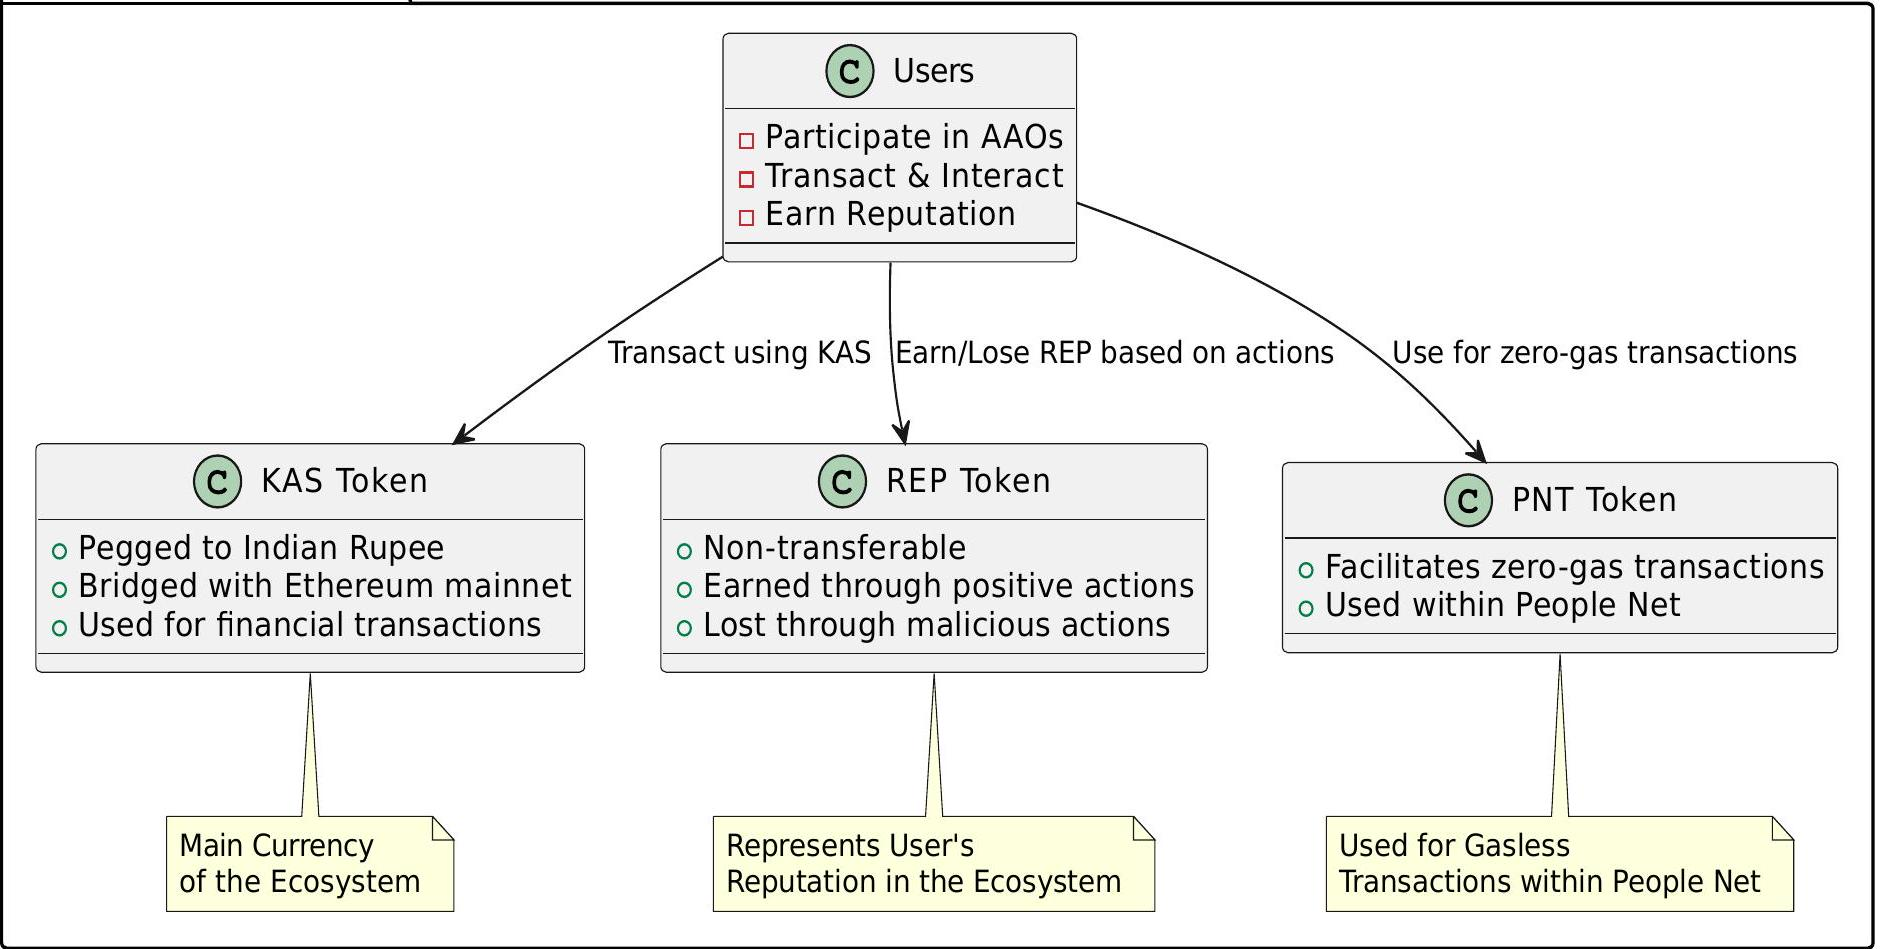
\includegraphics[max width=\textwidth, center]{2025_03_06_545dea0014012947d15fg-07}

Figure 6: Token flow and interactions within the PeopleNet ecosystem.

In conclusion, the tokenomics of PeopleNet is thoughtfully designed to ensure a balanced, fair, and efficient ecosystem, promoting positive behavior and facilitating seamless interactions.

\section*{8 Participation of People}
The PeopleNet ecosystem thrives on the active participation of its users. Unlike traditional systems where users are mere consumers, PeopleNet empowers individuals to take on various roles, contributing to the network's growth, security, and functionality.

\subsection*{8.1 Roles and Responsibilities}
\subsection*{8.1.1 Arbitrators}
Arbitrators play a crucial role in resolving disputes within the network, especially concerning exit problems in plasma chains. They ensure that the network remains fair and just.

\begin{itemize}
  \item Responsibilities: Reviewing evidence, listening to involved parties, and making unbiased decisions.
  \item Benefits: Earn REP tokens for their service, enhancing their reputation within the ecosystem.
\end{itemize}

\subsection*{8.1.2 Contributors}
Contributors add value to the network by offering services, creating content, or aiding in platform development.

\begin{itemize}
  \item Responsibilities: Delivering quality services, adhering to community guidelines, and actively engaging with the community.
  \item Benefits: Earn KAS tokens for their contributions and services.
\end{itemize}

\subsection*{8.1.3 Proposers}
Proposers initiate new projects, ideas, or AAOs, driving innovation and growth within the ecosystem.

\begin{itemize}
  \item Responsibilities: Presenting clear proposals, gathering support, and executing the proposed ideas.
  \item Benefits: Gain support in the form of KAS tokens or services from other participants.
\end{itemize}

\subsection*{8.1.4 Funders}
Funders provide the necessary financial support to projects or AAOs, ensuring their successful execution.

\begin{itemize}
  \item Responsibilities: Evaluating proposals, allocating funds wisely, and monitoring project progress.
  \item Benefits: Potential returns on successful projects and an increase in REP tokens for positive funding decisions.
\end{itemize}

\subsection*{8.1.5 Founders}
Founders establish new AAOs, setting the vision, mission, and goals for the organization.

\begin{itemize}
  \item Responsibilities: Leading the AAO, making strategic decisions, and ensuring the AAO's success.
  \item Benefits: Enhanced reputation within the ecosystem and potential KAS token rewards for successful AAO management.
\end{itemize}

\subsection*{8.2 Empowering the Masses}
PeopleNet's design ensures that every participant, regardless of their role, has a voice. The platform's decentralized nature, combined with its reputation system, ensures that good actors are rewarded, while malicious actors are deterred. This creates a selfregulating ecosystem where participants are incentivized to act in the best interests of the community.\\
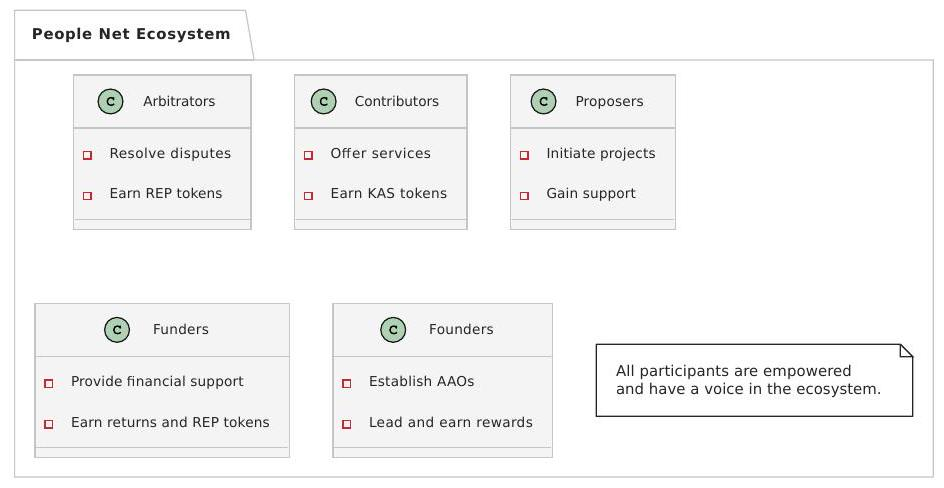
\includegraphics[max width=\textwidth, center]{2025_03_06_545dea0014012947d15fg-08}

Figure 7: Flow of roles and interactions within the PeopleNet ecosystem.

In conclusion, the active participation of people is the lifeblood of the PeopleNet ecosystem. By empowering individuals to take on various roles and\\
responsibilities, the platform fosters a vibrant, dynamic, and self-sustaining community.

\section*{9 Privacy and Data Security with PODs}
In the age of digital transformation, data privacy and security have become paramount [19]. With increasing concerns about data breaches, unauthorized access, and misuse of personal information, there's a pressing need for a system that prioritizes user data protection. PeopleNet, with its innovative use of Solid PODs, addresses these concerns head-on [2].

\subsection*{9.1 Understanding Solid PODs}
Solid, an acronym for "Social Linked Data", is a web decentralization project led by Prof. Tim BernersLee [2]. Its primary objective is to allow users to have full control over their data. PODs, or "Personal Online Data stores", are where this data is stored.

\begin{itemize}
  \item User Control: Each POD belongs to a user, ensuring they have complete control over their data.
  \item Decentralization: Data isn't stored in centralized servers but in individual PODs, reducing the risk of mass data breaches (12].
  \item Interoperability: PODs can be accessed by various apps with user permission, ensuring data portability and interoperability [5].
\end{itemize}

\subsection*{9.2 Implementation in PeopleNet}
PeopleNet takes the concept of Solid PODs and integrates it into its ecosystem to ensure maximum data privacy and security.

\subsection*{9.2.1 Dual POD System}
Each user in PeopleNet is provided with two PODs:

\begin{enumerate}
  \item Cryptographic POD: Acts as a cryptographic key, enabling network access. Stored both online and encrypted on the user's device [12].
  \item Data POD: Contains all user data, including interactions, media, and potentially a full node of their personal chain in the future.
\end{enumerate}

\subsection*{9.2.2 Data Ownership and Control}
All user-generated content, be it text, images, audio, or video, is stored in the Data POD. This ensures that users retain full ownership of their data, deciding who can access it and for what purpose [10].

\subsection*{9.2.3 Enhanced Security}
The decentralized nature of PODs, combined with encryption, ensures that user data is secure from breaches [12]. Even if an attacker gains access to one POD, the data of other users remains uncompromised.\\
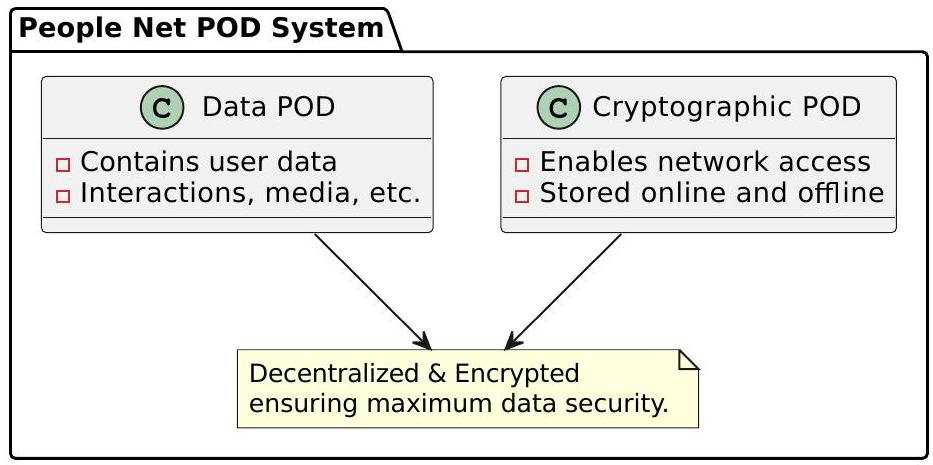
\includegraphics[max width=\textwidth, center]{2025_03_06_545dea0014012947d15fg-09}

Figure 8: Structure and security layers of the Solid PODs in PeopleNet.

\subsection*{9.3 Conclusion}
PeopleNet's integration of Solid PODs signifies a paradigm shift in how user data is perceived and managed. Instead of being mere data points in a centralized database, users are empowered, owning, and controlling their digital footprint. This not only enhances privacy but also fosters trust, a critical component for the widespread adoption of any digital platform (19].

\section*{10 Conclusion and the Future}
As we stand on the precipice of a new digital era, the importance of decentralization, privacy, and user empowerment cannot be overstated. The challenges of the current digital landscape, from data monopolies to the erosion of individual privacy, necessitate a transformative solution. PeopleNet, with its innovative architecture, AAOs, and emphasis on usercentricity, offers a beacon of hope in this context.

The vision of PeopleNet is not just about creating another blockchain platform. It's about ushering in a new digital society where individuals are not mere data points but active participants, shaping their digital destinies. By prioritizing user autonomy, decentralization, and transparency, PeopleNet seeks to redefine the very fabric of our online interactions.

The integration of Solid PODs ensures that users have unparalleled control over their data. The dual POD system, with its emphasis on encryption and decentralization, offers a robust shield against data breaches and unauthorized access. The AAOs, with their democratic ethos, pave the way for a more inclusive and participatory digital environment.

But beyond these technical aspects, at its core, PeopleNet is about people. It's about empowering the common man, bridging the digital divide, and ensuring that the fruits of the digital revolution are accessible to all, irrespective of socio-economic backgrounds. The project's focus on India, with its diverse and vast population, underscores this commitment to inclusivity.

As we look to the future, the potential of PeopleNet is boundless. From revolutionizing online governance to fostering digital communities where creativity and collaboration thrive, the possibilities are endless. The project's emphasis on incentivizing positive contributions and penalizing malicious actors ensures a digital ecosystem that is both vibrant and secure.

In conclusion, PeopleNet represents a bold step towards a decentralized digital future. A future where the power dynamics of the digital realm are upended, and users, not corporations, are in the driver's seat. As the project unfolds, it promises to be a transformative force, heralding a new age of digital democracy, empowerment, and innovation. The future is decentralized, and with PeopleNet, it's in the hands of the people.

\section*{References}
[1] Massimo Bartoletti and Livio Pompianu. "Burning for Money? Strategies and Potential Solutions to the Ethereum Gas Crisis". In: Journal of Computer Security (2019).\\[0pt]
[2] Tim Berners-Lee and Kieron O'Hara. "Redecentralizing the web, for good this time". In: Proceedings of the 29th ACM Conference\\
on Hypertext and Social Media. ACM. 2016, pp. 4-4.\\[0pt]
[3] Joseph Bonneau et al. "SoK: Research perspectives and challenges for Bitcoin and cryptocurrencies". In: (2015), pp. 104-121.\\[0pt]
[4] Vitalik Buterin et al. "Chain interoperability". In: 2016. URL: \href{https://allquantor}{https://allquantor} at/blockchainbib/pdf/buterin2016chain. pdf.\\[0pt]
[5] George Danezis and Sarah Meiklejohn. "Centrally banked cryptocurrencies". In: (2016).\\[0pt]
[6] Thang N. Dinh and My T. Thai. "Proof of Stake Blockchain: Performance and Scalability for Groupware Communications". In: IEEE INFOCOM 2018-IEEE Conference on Computer Communications (2018).\\[0pt]
[7] Jacob Eberhardt and Stefan Tai. "Or \&\# x201C; Where is my state? \&\# x201D;: Revisiting Ethereum storage". In: Proceedings of the ACM Workshop on Blockchain, Cryptocurrencies and Contracts. 2017, pp. 31-36.\\[0pt]
[8] Adem Efe Gencer et al. "Decentralization in Bitcoin and Ethereum Networks". In: Financial Cryptography and Data Security (2018).\\[0pt]
[9] Arthur Gervais et al. "On the Scalability and Security of Bitcoin". In: Distributed Computing Systems (ICDCS), 2016 IEEE 36th International Conference on (2016).\\[0pt]
[10] Glenn Greenwald. "NSA collecting phone records of millions of Verizon customers daily". In: The Guardian (2013).\\[0pt]
[11] Loi Luu et al. "Ethereum Smart Contracts: Security Vulnerabilities and Security Tools". In: Journal of Computer Security (2016).\\[0pt]
[12] Satoshi Nakamoto. "Bitcoin: A peer-to-peer electronic cash system". In: (2008). URL: https: \href{//bitcoin.org/bitcoin.pdf}{//bitcoin.org/bitcoin.pdf}.\\[0pt]
[13] Team Rocket. "Scalable and Probabilistic Leaderless BFT Consensus through Metastability". In: arXiv preprint arXiv:1902.06734 (2019).\\[0pt]
[14] Voshmgir Shermin. "A blockchain explanation your parents could understand". In: 2018. URL: \href{https://taylorpearson.me/blockchain}{https://taylorpearson.me/blockchain} -for-dummies/.\\[0pt]
[15] Don Tapscott and Alex Tapscott. Blockchain revolution: how the technology behind bitcoin is changing money, business, and the world. Penguin, 2016.\\[0pt]
[16] Polygon Team. "Polygon: A platform for Ethereum-compatible multi-chain networks". In: Whitepaper (2021).\\[0pt]
[17] Gavin Wood. "Ethereum: A secure decentralised generalised transaction ledger". In: (2014). URL: \href{https://ethereum.github.io/}{https://ethereum.github.io/} yellowpaper/paper.pdf.\\[0pt]
[18] Aviv Zohar. "Bitcoin: Under the hood". In: Communications of the ACM 58.9 (2015), pp. 104-113.\\[0pt]
[19] Shoshana Zuboff. "The age of surveillance capitalism: The fight for a human future at the new frontier of power". In: Public Affairs (2019).


\end{document}